\section{Discussion of Physics Implications}
\label{sec:discussion}

One very comprehensive (and therefore representative) studies of the pre-LHC data is by the COMPETE collaboration \cite{compete}. In total 256 models, all without crossing-odd components, were considered to describe $\sigma_{\rm tot}$ and $\rho$ data for various reactions ($\rm pp$, $\rm p\pi$, $\rm pK$, etc.) and the corresponding particle-antiparticle reactions. Out of these models, 23 were found to give a reasonable description of the data \cite{compete-details}. Extrapolations from these models are confronted with newer TOTEM measurements in Figure~\ref{fig:comp bands}, which shows that they are grouped in 3 bands. Each band is plotted in a different colour and has a different level of compatibility with the data. As argued above, the $13\un{TeV}$ fit with $N_b=1$ and $|t|_{\rm max} = 0.07\un{GeV^2}$ (rightmost point in the figure) corresponds to the most fair comparison to past analyses and is therefore used to evaluate the compatibility with the COMPETE models. The $8\un{TeV}$ $\rho$ point is not included in this calculation since it does not bring any information due to its large uncertainty. The $\sigma_{\rm tot}$ measurements can be, to a large extent, regarded as independent: they used data from different LHC fills at different energies, different beam optics, often different RPs, often different analysis approaches (fit parametrisation, treatment of CNI) and often they were analysed by different teams. The only correlation comes from using common normalisation at a given collision energy. Consequently, two compatibility evaluations were made: using all $\sigma_{\rm tot}$ points from Figure~\ref{fig:comp bands} and using their subset with a single point per energy. These two results thus provide upper and lower bounds for the actual compatibility level. The observations can be summarised as follows.
\begin{itemize}[noitemsep,topsep=0pt]
\item The blue band is compatible (p-value $0.990$ to $0.995$) with the $\sigma_{\rm tot}$ data, but incompatible (p-value $3\times10^{-6}$) with the $\rho$ point.
\item The magenta band is incompatible (p-value $1\times10^{-5}$ to $5\times10^{-4}$) with the $\sigma_{\rm tot}$ data and incompatible (p-value $9\times10^{-3}$) with the $\rho$ point.
\item The green band is incompatible (p-value $3\times10^{-18}$ to $5\times10^{-12}$) with the $\sigma_{\rm tot}$ data, but compatible (p-value $0.4$) with the $\rho$ point.
\end{itemize}
In summary, none of the COMPETE models is compatible with the ensemble of TOTEM's $\sigma_{\rm tot}$ and $\rho$ measurements.

\begin{figure*}
\vskip-5mm
\begin{center}
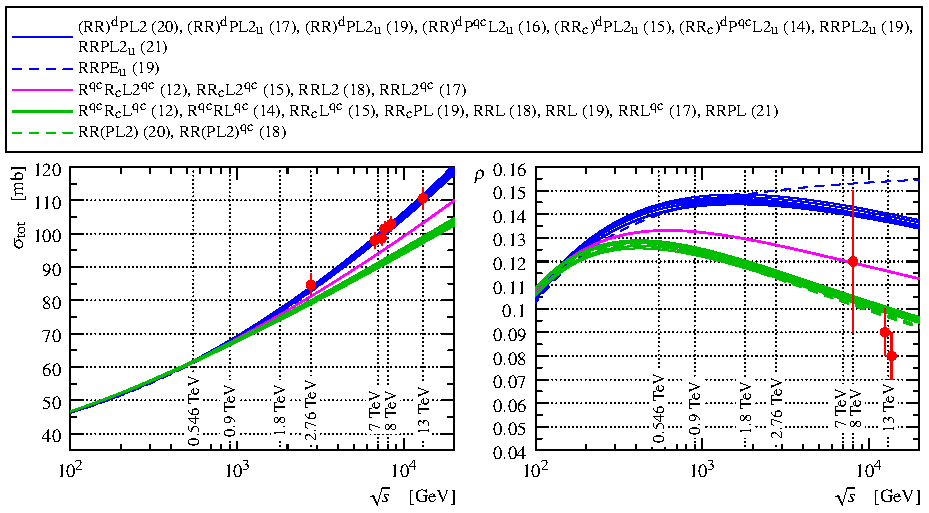
\includegraphics{fig/compete_bands_si_tot_rho.pdf}
\caption{%
Predictions of COMPETE models \cite{compete-details} for $\rm pp$ interactions. Each model is represented by one line (see legend). The red points represent the reference TOTEM measurements. The $\sigma_{\rm tot}$ point at $13\un{TeV}$ corresponds to the weighted average in Eq.~(\ref{eq:si tot comb}). The two $\rho$ points at $13\un{TeV}$ correspond to the two cases discussed in Section~\ref{sec:rho anal}: the left point to the fit with $N_b=3$ and $|t|_{\rm max} = 0.15\un{GeV^2}$, the right point to $N_b=1$ and $|t|_{\rm max} = 0.07\un{GeV^2}$.
}
\label{fig:comp bands}
\end{center}
\end{figure*}

Another, even less model-dependent, relation between $\sigma_{\rm tot}$ and $\rho$ can be obtained from dispersion relations \cite{dremin-dispersion,barone-predazzi}. If only the crossing-even component of the amplitude is considered, it can be shown that $\rho$ is proportional to the rate of growth of $\sigma_{\rm tot}$ with energy. Therefore, the low value of $\rho$ determined in Section~\ref{sec:rho} indicates that either the total cross-section growth should slow down at higher energies or that there is a need for an odd-signature object being exchanged by the protons. While at lower energies such contributions may naturally come from secondary Reggeons, their contribution is generally considered negligible at LHC energies due to their Regge trajectory intercept lower than unity.

A variety of odd-signature exchanges relevant at high energies have been discussed in literature, within different frameworks and under different names, see e.g.~the reviews \cite{braun,ewerz}. The ``Odderon'' was introduced within the axiomatic theory \cite{nicolescu-1973,nicolescu-1992,nicolescu-2007} as an amplitude contribution responsible for $\rm p\bar p$ vs.~$\rm pp$ differences in the total cross-section as well as in the differential cross-section, particularly in the dip region. Crossing-odd trajectories were also studied within the framework of Regge theory as a counterpart of the crossing-even Pomeron. It has also been shown that an such object must exist in QCD, as a colourless bound state of three gluons with quantum numbers $J^{PC} = 1^{--}$ (see e.g.~\cite{bartels-2000}). The binding strength among the 3 gluons is greater than the strength of their interaction with other particles. There is also evidence for such a state in QCD lattice calculations, known under the name ``vector glueball'' (see e.g.~\cite{morningstar-1999}). Such a state, on one hand, can be exchanged in the $t$-channel and contribute, e.g., to the elastic-scattering amplitude. On the other hand it can be created in the $s$-channel and thus be observed in spectroscopic studies. Non-perturbative QCD studies based on the AdS/CFT correspondence show that the Odderon emerges on equally firm footing as the Pomeron \cite{brower-2009}.

There are multiple ways how an odd-signature exchange component may manifest itself in observable data. Focussing on elastic scattering at the LHC (unpolarised beams), there are 3 regions often argued to be sensitive. In general, the effects of an odd-signature exchange (3 bound gluons) are expected to be much smaller than those of even-signature exchanges (2 bound gluons). Consequently, the sensitive regions are those where the contributions from 2-bound-gluon exchanges cancel or are small. At very low $|t|$ the 2-bound-gluon amplitude is expected to be almost purely imaginary, while a 3-gluon exchange would make contributions to the real part and therefore $\rho$ is a very sensitive parameter. Another such example is the dip, often described as the imaginary part of the amplitude crossing zero, thus ceding the dominance to the real part to which a 3-gluon exchange may contribute. In agreement with such predictions, the observed dips in $\rm p\bar p$ scattering are shallower than those in $\rm pp$. At $\sqrt s = 53\un{GeV}$, there are data showing a very significant difference between the $\rm pp$ and $\rm p\bar p$ dip \cite{breakstone-85}. The interpretation of this difference is, however, complicated due to non-negligible contribution from secondary Reggeons. These are not expected to give sizeable effects at the Tevatron energies, which thus gives weight to the D0 observation of a very shallow dip in $\rm p\bar p$ elastic scattering \cite{d0-elastic} compared to the very pronounced dip measured by TOTEM at $7\un{TeV}$ \cite{totem-7tev-first}. The $\rm pp$ vs.~$\rm p\bar p$ dip difference is also predicted to be energy-dependent which presents another experimental observable (see e.g.~\cite{ster-2015}). Sometimes the high-$|t|$ region is also argued to be sensitive to 3-gluon exchanges since the contribution from 2-gluon exchanges is rapidly dropping. However, preliminary high-$|t|$ TOTEM data at $13\un{TeV}$ indicate that this region is dominated by a perturbative-QCD amplitude, e.g.~\cite{Donnachie:1979yu}.

\begin{figure*}
\vskip-5mm
\begin{center}
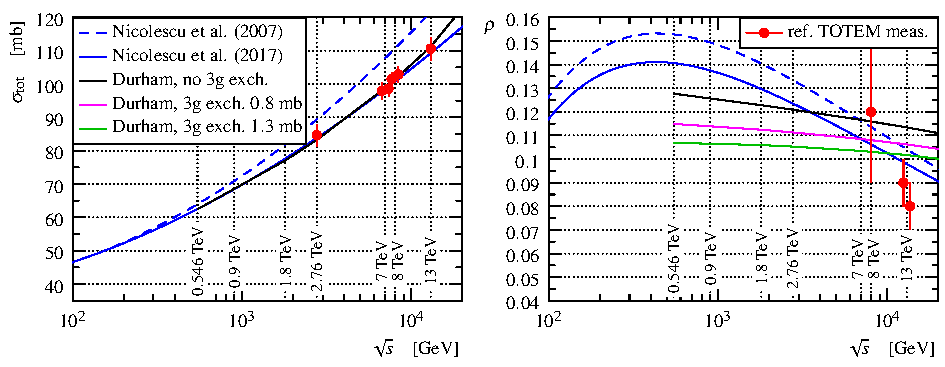
\includegraphics{fig/matching_models_si_tot_rho.pdf}
\caption{%
Predictions of the model by Nicolescu et al.~(dashed blue curve from \cite{nicolescu-2007}, solid blue curve from \cite{nicolescu-2017}) and the Durham model \cite{durham-2018} (including crossing-odd contribution from \cite{levin-1990}) compared to the reference TOTEM measurements (red dots). The $\sigma_{\rm tot}$ point at $13\un{TeV}$ corresponds to the weighted average in Eq.~(\ref{eq:si tot comb}). The two $\rho$ points at $13\un{TeV}$ correspond to the two cases discussed in Section~\ref{sec:rho anal}: the left point to the fit with $N_b=3$ and $|t|_{\rm max} = 0.15\un{GeV^2}$, the right point to $N_b=1$ and $|t|_{\rm max} = 0.07\un{GeV^2}$. For the Durham model the black curve corresponds to the prediction without a colourless 3-gluon $t$-channel exchange. The magenta and green curves refer to the $\rm pp$ predictions including a 3-gluon exchange with proton coupling equivalent to $0.8$ and $1.3\un{mb}$, respectively.
}
\label{fig:match models}
\end{center}
\end{figure*}

Figure~\ref{fig:match models} compares the TOTEM data with two compatible models: by Nicolescu et al.~\cite{nicolescu-2017} and the extended Durham model \cite{durham-2018} (original model \cite{durham-2014} plus crossing-odd contribution from \cite{levin-1990}). The 2007 version of the Nicolescu model (dashed blue) is based only on pre-LHC data and predicts $\sigma_{\rm tot}$ overestimating the TOTEM measurements -- as argued in Ref.~\cite{nicolescu-2017} it might be due to the ambiguities in prolonging the amplitudes in the non-forward region. The 2017 version (solid blue) includes also LHC measurements up to $13\un{TeV}$ and describes the $\sigma_{\rm tot}$ data well. Both versions yield similar results for $\rho$, with a pronounced energy dependence. This comes from the fact that the crossing-odd component is almost negligible at $\sqrt s \approx 500\un{GeV}$ but very significant at $13\un{TeV}$. Conversely, in the Durham model the effect is sizeable at $\sqrt s \approx 500\un{GeV}$ and gently diminishes with energy. The Durham model also predicts a mild energy dependence of the $\rho$ parameter. Therefore, precise $\rho$ measurements at $\sqrt s \approx 900\un{GeV}$ and $14\un{TeV}$ would be valuable for discrimination between these models. For both models, the inclusion of a crossing-odd exchange component was essential to reach the agreement between the data and model. In particular, the Durham model without such a contribution (black line) is not well compatible (p-value $0.02$) with the (rhs.) $\rho$ point obtained with $N_b=1$ and $|t|_{\rm max} = 0.07\un{GeV^2}$.
